\documentclass[a4paper,11pt]{article}
\usepackage[utf8]{inputenc}
\usepackage{amsmath, amssymb}
\usepackage{geometry}
\usepackage{pgfplots}
\pgfplotsset{compat=1.18}

\geometry{margin=1.5cm}

\title{Fiche : Équations Différentielles Linéaires}
\author{Raphaël Jamann}
\date{}

\begin{document}

    \maketitle

    \section*{Équations différentielles linéaires d'ordre 1}

        \subsection*{Forme générale}
            Une équation différentielle linéaire du premier ordre s'écrit :
            \[
            y'(x) + a(x)y(x) = b(x)
            \]

        \subsection*{Cas homogène}
            \[
            y'(x) + a(x)y(x) = 0
            \]

            \textbf{Solution générale :}
            \[
            y(x) = C e^{-\int a(x)\,dx}
            \]

        \subsection*{Cas non homogène}
            \[
            y'(x) + a(x)y(x) = b(x)
            \]

            \textbf{Méthode : facteur intégrant}

            \begin{itemize}
                \item Facteur intégrant :
                \[
                \mu(x) = e^{\int a(x)\,dx}
                \]
                \item Solution générale :
                \[
                y(x) = \frac{1}{\mu(x)} \left( \int \mu(x)b(x)\,dx + C \right)
                \]
            \end{itemize}

        \subsection*{Structure des solutions}
            \[
            y = y_h + y_p
            \]
            où :
            \begin{itemize}
                \item $y_h$ : solution de l'équation homogène
                \item $y_p$ : une solution particulière
            \end{itemize}

        \newpage

    \section*{Équations différentielles linéaires d'ordre 2}

        \subsection*{Forme générale}
            \[
            y'' + ay' + by = f(x)
            \]
            avec $a, b$ constants.

        \subsection*{Équation homogène associée}
            \[
            y'' + ay' + by = 0
            \]

        \subsection*{Équation caractéristique}
            \[
            r^2 + ar + b = 0
            \]

        \subsection*{Selon le discriminant $\Delta = a^2 - 4b$}

            \subsubsection*{1. $\Delta > 0$ - Régime sur-amorti}
                
                $$ r_1, r_2 \in \mathbb{R}$$
                
                $$ y_h (t) = A e^{r_1 t} + B e^{r_2 t}, \quad A, B \in \mathbb{R} $$

                \begin{center}
                    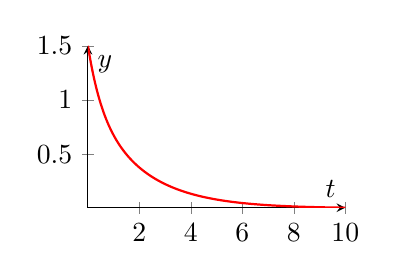
\begin{tikzpicture}
                        \begin{axis}[
                            domain=0:10,
                            samples=200,
                            axis lines=middle,
                            xlabel=$t$,
                            ylabel=$y$,
                            width=0.4\textwidth,
                            height=0.3\textwidth
                        ]
                        \addplot[no markers, smooth, thick, color=red] {exp(-0.5*x) + 0.5*exp(-2*x)};
                        \end{axis}
                    \end{tikzpicture}
                \end{center}

            \subsubsection*{2. $\Delta = 0$ - Régime critique}
                $$ r \in \mathbb{R} $$
                $$ y_h (t) = (A + B t)e^{rt}, \quad A, B \in \mathbb{R} $$


                \begin{center}
                    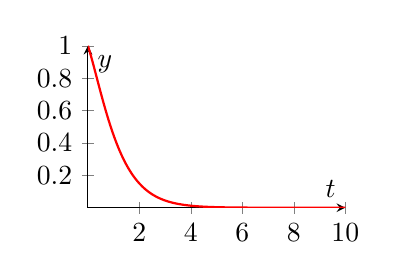
\begin{tikzpicture}
                        \begin{axis}[domain=0:10, samples=100, axis lines=middle, xlabel=$t$, ylabel=$y$, width=0.4\textwidth, height=0.3\textwidth]
                            \addplot[no markers, smooth, thick, color=red] {(1 + x)*exp(-1.5*x)};
                        \end{axis}
                    \end{tikzpicture}
                \end{center}

            \subsubsection*{3. $\Delta < 0$ - Oscillations libres amorties}
                $$ r = \alpha \pm i\beta \in \mathbb{C} $$
                $$ y_h (t) = e^{\alpha t}(C_1 \cos \beta t + C_2 \sin \beta t) $$

                Exemple : $y'' + 2\delta y'+ \omega_0^2 y = 0$ 

                Solution : $y = e^{-\delta t} \left( A \cos (\omega t) + B \sin (\omega t) \right), \quad \omega = \sqrt{\omega_0^2 - \delta^2}$

                \begin{center}
                    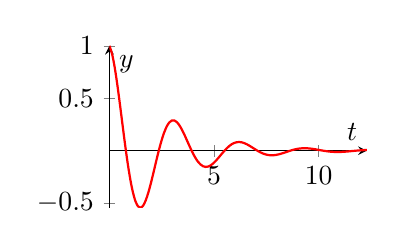
\begin{tikzpicture}
                        \begin{axis}[domain=0:12.3, samples=100, axis lines=middle, xlabel=$t$, ylabel=$y$,
                            width=0.4\textwidth,
                            height=0.3\textwidth
                        ]
                        \addplot[no markers, smooth, thick, color=red] {exp(-0.4*x)*cos(deg(2*x))};
                        \end{axis}
                    \end{tikzpicture}
                \end{center}

            \subsection*{Cas non homogène}

                \[
                y'' + ay' + by = f(x)
                \]

                \textbf{Solution générale :}
                \[
                y = y_h + y_p
                \]

        \subsection*{Recherche d'une solution particulière}

            Selon la forme de $f(x)$ :

            \begin{itemize}
                \item Polynôme $\rightarrow$ solution polynomiale
                \item Exponentielle $\rightarrow$ $Ae^{\lambda x}$ si $\lambda$ n'est pas solution de l'équation caractéristique,
                $A\lambda e^{\lambda x}$ si $\lambda$ est racine simple et $A\lambda^2 e^{\lambda x}$ si $\lambda$ est racine double.
                \item Sinus/Cosinus $\rightarrow$ $A\cos t + B\sin t$ \quad ou alors on passe par $\Re \left( e^{i\omega t} \right)$ pour $\cos$ et $\Im \left( e^{i\omega t} \right)$.
            \end{itemize}


        \subsection*{Résumé méthode}

            \begin{enumerate}
                \item Résoudre l'équation homogène (équation caractéristique)
                \item Trouver une solution particulière $y_p$
                \item Écrire la solution générale :
                \[
                y = y_h + y_p
                \]
            \end{enumerate}


\end{document}